% Section 05: Model Validation and Posterior Predictive Checks
\section{Model Validation: Posterior Predictive Checks}

To assess the reliability of our inferred parameters, we performed a Posterior Predictive Check (PPC) \parencite{beaumont2002approximate}.
This involved sampling 100 parameter sets $(\beta, \gamma, \rho)$ from the adjusted posterior distribution and re-simulating the epidemic process to see if the synthetic data could replicate the observed targets.

\subsection{Visual Inspection of Predictive Performance}

Figure \ref{fig:ppc_plots} presents the results of the PPC for the two primary data targets: the epidemic curve and the final degree distribution.
The faint lines represent 100 individual forward simulations from the posterior, while the dashed orange line represents the observed data.

\begin{figure}[H]
    \centering
    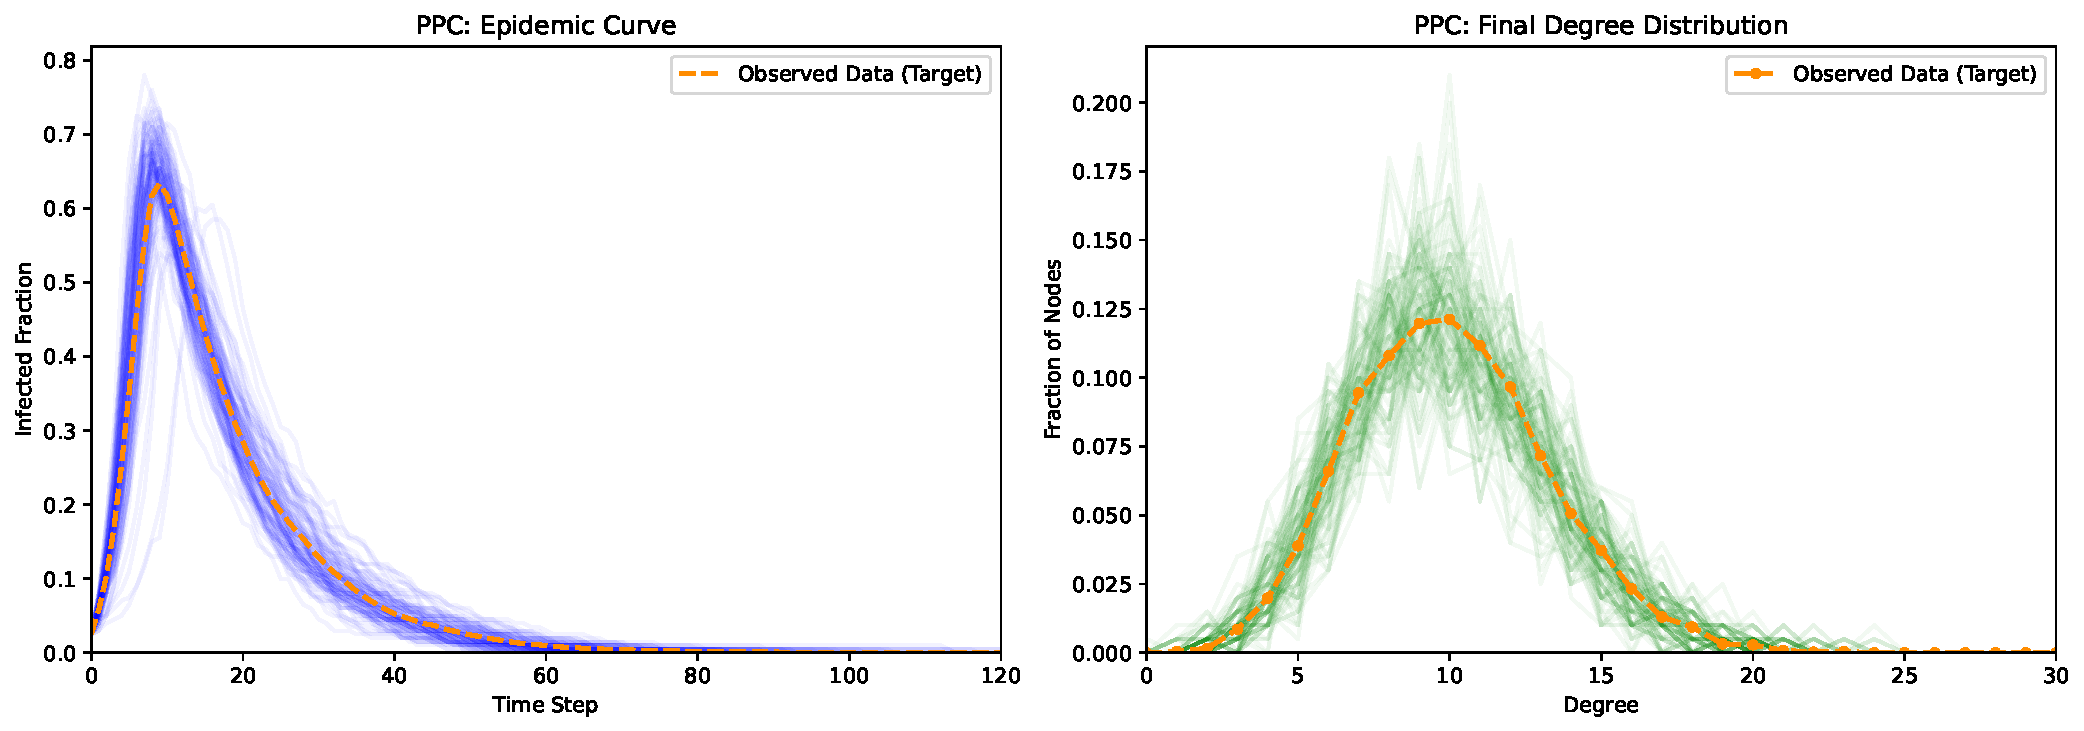
\includegraphics[width=0.95\textwidth]{plots/smc_abc_ppc_plot.pdf}
    \caption{Posterior Predictive Checks (PPC). Left: The observed epidemic curve (orange) is perfectly centered within the ensemble of posterior simulations (blue). Right: The observed final degree distribution (orange) aligns closely with the predicted topological structures (green).}
    \label{fig:ppc_plots}
\end{figure}

The visual alignment is exceptional.
The observed trajectory is entirely contained within the predictive ensemble, indicating that our posterior distribution is not only precise but also accurately captures the stochastic variations of the underlying model.

\subsection{Quantitative Performance Metrics}

To rigorously quantify the model fit, we calculated the 95\% Prediction Interval (PI) coverage and the Root Mean Square Error (RMSE) between the mean of the posterior predictions and the observed data.
The results are summarized in Table \ref{tab:ppc_results}.

\begin{table}[H]
\centering
\caption{Quantitative PPC Performance Metrics}
\label{tab:ppc_results}
\begin{tabular}{lcc}
\toprule
Metric & 95\% PI Coverage & Prediction Error (RMSE) \\
\midrule
Epidemic Curve (Infected Fraction) & 100.0\% & 0.00455 \\
Final Degree Distribution & 100.0\% & 0.00190 \\
\bottomrule
\end{tabular}
\end{table}

The 100\% coverage for both the temporal (infection) and structural (network) statistics confirms that the true parameters are highly likely to be contained within our inferred posterior.
Furthermore, the extremely low RMSE values (e.g., $0.00455$ for infection fraction) suggest that our "best-fit" estimates can replicate the observed data with near-perfect accuracy.

These validation results provide strong evidence that the integration of Mahalanobis distance and local linear regression successfully resolved the parameter identification challenges inherent in adaptive network models.